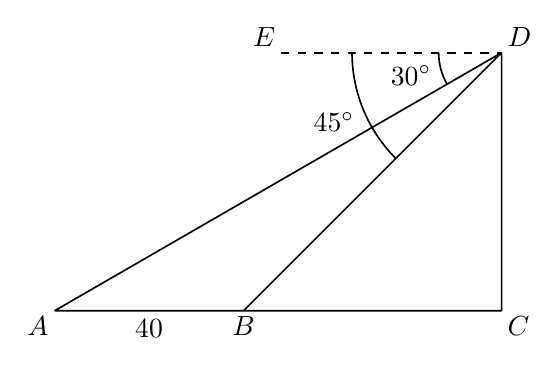
\begin{tikzpicture}[x=1cm,y=1cm,font=\normalsize,
 geometry edge/.style={solid,line width=.6pt},
 geometry mark/.style={solid,line width=.6pt},
 geometry label/.style={font=\normalsize,inner sep=0pt}]

% scale .06 cm per metre; AB=40; depression angles 30 and 45 degrees.
\coordinate (C) at (0,0);
\coordinate (D) at (0,3.278460969083);
\coordinate (B) at (-3.278460969083,0);
\coordinate (A) at (-5.678460969083,0);
\coordinate (E) at (-2.8,3.278460969083);
\draw[geometry edge,dashed] (E)--(D);
\draw[geometry edge] (D)--(A) (D)--(B) (D)--(C) (A)--(C);
\draw[geometry mark] (D) ++(180:8mm) arc[start angle=180,end angle=210,radius=8mm];
\draw[geometry mark] (D) ++(180:19mm) arc[start angle=180,end angle=225,radius=19mm];
\node[inner sep=0pt] at (-1.15,2.988460969083) {$30^\circ$};
\node[inner sep=0pt] at (-2.13,2.398460969083) {$45^\circ$};
\node[geometry label,below left=2pt] at (A) {$A$};
\node[geometry label,below=2pt] at (B) {$B$};
\node[geometry label,below right=2pt] at (C) {$C$};
\node[geometry label,above right=2pt] at (D) {$D$};
\node[geometry label,above left=2pt] at (E) {$E$};
\node[below=3pt,inner sep=0pt] at (-4.478460969083,0) {$40$};
\end{tikzpicture}
